\section{Grundlagen zu linearen Gleichungssystemen}

\stepcounter{subsection}% Im Original steht vor den Beispielen kein eigener Unterabschnitt (Nummerierung 1.1.1.x)

Zur Einführung in die Thematik folgt ein Beispiel.

\subsubsection{Beispiel}

Eine Firma produziert 2 Produkte $P_1$ und $P_2$. Durch Messungen in der laufenden Produktion ist bekannt, dass bei der Herstellung von 13 Produkten $P_1$ und 4 Produkten $P_2$ ein Energiebedarf von 190\,kWh nötig ist und bei 3 Produkten von $P_1$ und 1 Produkt von $P_2$ ein Energiebedarf von 45\,kWh.

Wie groß ist der Energiebedarf zur Herstellung jedes einzelnen Produktes?

Zur Beantwortung dieser Frage bezeichnet man mit $x_1$ den Energiebedarf pro Stück zur Produktion von $P_1$ und mit $x_2$ den Energiebedarf pro Stück zur Produktion von $P_2$. Es ergeben sich nun zwei Gleichungen:
\begin{align*}
  13x_1 + 4x_2 &= 190 \qquad \text{I}\\
  3x_1 + x_2 &= 45 \qquad \text{II}
\end{align*}
Gesucht sind also Werte für $x_1$ und $x_2$, die sowohl Gleichung I als auch Gleichung II erfüllen.

Sowohl in Gleichung I wie in II erscheinen $x_1$ und $x_2$ nur in einfacher Potenz (siehe auch den Abschnitt über lineare Gleichungen in Lerneinheit 1). Da es sich folglich um ein System von \emph{linearen} Gleichungen handelt, spricht man von einem \textbf{linearen Gleichungssystem} (\textit{LGS}) mit zwei Gleichungen in zwei Unbekannten $x_1$ und $x_2$.

Zum Lösen eines LGS stehen verschiedene Methoden (Algorithmen) zur Verfügung.

Für das LGS oben können wir das \textbf{Einsetzungsverfahren} anwenden. Dazu stellen wir zunächst in Gleichung II die Unbekannte $x_2$ frei:
\[ x_2 = 45 - 3x_1 \]
Diese wird in Gleichung I eingesetzt:
\begin{align*}
  13x_1 + 4(45 - 3x_1) &= 190\\
  x_1 &= 10
\end{align*}
Mit dem Wert für $x_1$ berechnet sich schließlich $x_2 = 15$. Der Energiebedarf zur Produktion von $P_1$ beträgt also 10\,kWh, der Energiebedarf zur Produktion von $P_2$ beträgt 15\,kWh.

Vom mathematischen Standpunkt aus ist wesentlich: Allein das Wertepaar $x_1 = 10$ und $x_2 = 15$ erfüllt beide Gleichungen und damit das Gleichungssystem. Die Lösung ist also eindeutig nur das Paar $(10;15)$.\beispielende

Statt des \textbf{Einsetzungsverfahrens} hätte man in dem Beispiel auch das \textbf{Additionsverfahren} verwenden können. Letzteres basiert auf der Grundidee, die auch dem \textbf{Gauß-Verfahren} (dazu später mehr) zugrunde liegt: Man addiert und subtrahiert die gegebenen Gleichungen so geschickt voneinander, dass dabei Unbekannte heraus fallen und die übrig bleibenden Unbekannten direkt berechnet werden können.

Für das obige Beispiel funktioniert das so: Ausgehend von dem Gleichungssystem
\begin{align*}
  13x_1 + 4x_2 &= 190 \qquad \text{I}\\
  3x_1 + x_2 &= 45 \qquad \text{II}
\end{align*}
multipliziert man die zweite Gleichung mit $\tfrac{13}{3}$, damit auch bei dieser der Koeffizient 13 vor $x_1$ steht. Das neue Gleichungssystem lautet:
\begin{align*}
  13x_1 + 4x_2 &= 190 \qquad \text{I}\\
  13x_1 + \tfrac{13}{3}x_2 &= 195 \qquad \text{II}'
\end{align*}
Jetzt kann man die erste Gleichung von der zweiten subtrahieren, das Ergebnis ist eine neue zweite Gleichung, und man erhält:
\begin{align*}
  13x_1 + 4x_2 &= 190 \qquad \text{I}\\
  \tfrac{1}{3}x_2 &= 5 \qquad \text{II}''
\end{align*}
Nun kann man -- und das war der Sinn der ganzen Übung -- aus der neuen zweiten Gleichung das Ergebnis $x_2 = 15$ direkt ablesen! Setzt man dies nun noch in die erste Gleichung ein, ergibt sich sofort $x_1 = 10$. Die richtige Lösung wurde also auch auf diese Weise gefunden!

Ein weiteres Lösungsverfahren für LGS mit nur zwei Unbekannten $x_1$ und $x_2$ ist die \textbf{grafische Ermittlung der Lösung}.

Dazu wird noch einmal unser LGS mit zwei Gleichungen und zwei Unbekannten betrachtet:
\begin{align*}
  13x_1 + 4x_2 &= 190 \qquad \text{I}\\
  3x_1 + x_2 &= 45 \qquad \text{II}
\end{align*}
Einer Gleichung mit zwei Unbekannten ist eine Gerade zugeordnet. Schreibt man nämlich $x$ statt $x_1$ und $y$ statt $x_2$, so lautet die erste Gleichung nun
\[ 13x + 4y = 190 \]
oder nach $y$ aufgelöst:
\[ y = -\frac{13}{4}x + \frac{190}{4} \]
Dies ist die Gleichung einer Geraden $g_1$ im $x$-$y$-Koordinatensystem! Die zweite Gleichung ergibt:
\[ y = -3x + 45 \]
Die zugehörige Gerade nennen wir $g_2$.

\begin{center}
  \begin{tikzpicture}
    \begin{axis}[width=10cm, height=7cm, axis lines=left, xmin=0, xmax=20.5, ymin=-12, ymax=55,
      xtick={2,4,...,20}, ytick={-10,10,...,50}, xlabel={$x$}, ylabel={$y$}, tick label style={font=\footnotesize}, samples=50]
      \addplot[black, thick, domain=0:20] {-13/4*x+190/4};
      \addplot[black, dashed, thick, domain=0:20] {-3*x+45};
    \end{axis}
  \end{tikzpicture}
\end{center}

Lösungen des LGS sind die Koordinaten $(x;y)$ der Punkte, die auf \emph{beiden} Geraden liegen. Die zwei Geraden schneiden sich genau in einem Punkt. Der Schnittpunkt hat die Koordinaten $(x;y) = (x_1;x_2) = (10;15)$. (Zugegebenermaßen ist dies in dem Schaubild nicht gut zu erkennen.)

Eine ebenfalls gebräuchliche Schreibweise ist:
\[ \begin{pmatrix} x_1 \\ x_2 \end{pmatrix} = \begin{pmatrix} 10 \\ 15 \end{pmatrix} \]

Das LGS besitzt genau eine Lösung. Generell stellt sich die Frage: Wie viele Zahlenpaare $(x_1;x_2)$ gibt es, die LGS mit zwei Gleichungen und zwei Unbekannten erfüllen? Existieren Gleichungssysteme, für die es keine, genau eine, drei, siebenundzwanzig oder unendlich viele Lösungen gibt?

Interessanterweise gilt für LGS die folgende mathematische Tatsache:
\merkbox{Ein LGS besitzt entweder keine, genau eine oder unendlich viele Lösungen.}

Wie die letzte grafische Betrachtung nahe legt, lässt sich auch diese allgemeine Tatsache für Gleichungssysteme mit zwei Unbekannten gut veranschaulichen. Dazu werden zwei weitere Gleichungssysteme mit zwei Gleichungen und zwei Unbekannten betrachtet:
\begin{center}
  \begin{tabular}{lcll}
    A: & $2x - y = 1$ & I & \\
       & $4x - 2y = 2$ & II & \\[6pt]
    B: & $2x - y = 1$ & I & \\
       & $4x - 2y = 3$ & II &
  \end{tabular}
\end{center}
Folgende Grafiken gehören zu den Gleichungssystemen.

\begin{center}
  \begin{tikzpicture}
    \begin{axis}[width=7cm, height=6cm, axis lines=middle, xmin=-4.3, xmax=4.3, ymin=-9, ymax=8,
      xtick={-4,...,4}, ytick={-8,-6,...,6}, xlabel={$x$}, ylabel={$y$}, tick label style={font=\tiny}, samples=50, title={Zu A:}]
      \addplot[black, thick, domain=-4:4] {2*x-1};
      \addplot[black, dashed, thick, domain=-4:4] {2*x-1};
    \end{axis}
  \end{tikzpicture}
  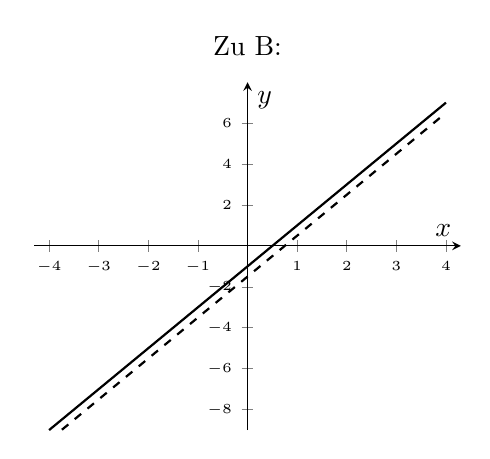
\begin{tikzpicture}
    \begin{axis}[width=7cm, height=6cm, axis lines=middle, xmin=-4.3, xmax=4.3, ymin=-9, ymax=8,
      xtick={-4,...,4}, ytick={-8,-6,...,6}, xlabel={$x$}, ylabel={$y$}, tick label style={font=\tiny}, samples=50, title={Zu B:}]
      \addplot[black, thick, domain=-4:4] {2*x-1};
      \addplot[black, dashed, thick, domain=-4:4] {2*x-1.5};
    \end{axis}
  \end{tikzpicture}
\end{center}

LGS A besitzt unendlich viele Lösungen, nämlich genau die Punkte, die auf beiden Geraden liegen. Da die Geraden identisch sind (die beiden Gleichungen beschreiben dieselbe Gerade!), gilt dies für alle Punkte der Geraden. Einige Lösungen sind:
\[ (x;y) = (0;-1), \quad (x;y) = (5;9), \quad (x;y) = (-1;-3) . \]
Überprüfen Sie die Lösungen, und geben Sie weitere an.

Dagegen besitzt LGS B keine Lösung, denn die parallelen Geraden besitzen keinen gemeinsamen Schnittpunkt.

Wie man an LGS A sieht, können unterschiedliche Gleichungen eines LGS äquivalent sein, d.\,h. die eine ist nur eine Umformung der anderen. Damit ist eine Gleichung des LGS »überflüssig«, sie trägt keine neuen Bedingungen zur Lösung bei. Gerade bei großen Gleichungssystemen mit vielen Unbekannten ist die Äquivalenz von Gleichungen nicht immer auf den ersten Blick zu erkennen!

Noch einmal zusammengefasst: Da zwei Geraden im $x$-$y$-Koordinatensystem entweder identisch oder parallel sind oder sich in genau einem Punkt schneiden, ist unmittelbar einsichtig, dass -- wie oben bereits gesagt -- ein LGS aus zwei Gleichungen mit zwei Unbekannten entweder unendlich viele, keine oder genau eine Lösung hat. Dies gilt sogar immer, d.\,h. für beliebig viele Gleichungen mit beliebig vielen Unbekannten! (Allerdings kann man es sich im allgemeinen Fall nicht mehr grafisch veranschaulichen.)

\subsubsection{Übungsaufgabe}

\begin{graukasten}
  a) Notieren Sie einige Lösungen zu dem (untypischen) LGS mit zwei Unbekannten und nur einer Gleichung:
  \[ 6x_1 + 12x_2 = -6 \]
  »Lösen« Sie das LGS grafisch, und überprüfen Sie Ihre berechneten Lösungen.

  b) Bestimmen Sie die möglichen Lagen dreier Geraden zueinander, und überlegen Sie, welche Aussagen über die Anzahl Lösungen des dazu gehörigen LGS getroffen werden können. (Es gibt 6 verschiedene Lagen der Geraden zueinander.)
\end{graukasten}

Das Ziel ist nun, ein allgemein gültiges, detailliertes Lösungsverfahren, also einen \textbf{Algorithmus}, für LGS zu bestimmen. Der Algorithmus muss folgende Fragen beantworten:
\begin{itemize}
  \item Wie viele Lösungen gibt es, d.\,h. gibt es keine Lösung, eine Lösung oder unendlich viele Lösungen?
  \item Wie berechne ich die Lösungen?
\end{itemize}
Der in Kürze vorgestellte Algorithmus ist eine Verallgemeinerung des Additionsverfahrens, d.\,h. er basiert darauf, dass in geschickter Weise so Gleichungen addiert und voneinander subtrahiert werden, dass die Lösungen leicht abgelesen werden können.
Der Vorbereitung dient ein weiteres Beispiel.

\subsubsection{Beispiel}

Das folgende LGS sei gegeben:
\begin{align*}
  x_1 - 2x_2 + x_3 &= 5 \qquad \text{I}\\
  -5x_1 - 2x_2 - x_3 &= -21 \qquad \text{II}\\
  6x_1 + 2x_2 - x_3 &= 16 \qquad \text{III}
\end{align*}

Wir gehen bei diesem Beispiel sehr langsam und Schritt für Schritt vor. Wenn man etwas mehr Übung hat, kann man auch mehrere Schritte gleichzeitig vollziehen.

Jetzt geht es los. Damit bei der zweiten und dritten Gleichung $x_1$ verschwindet, addiert man zur zweiten das 5-fache der ersten (und erhält damit eine neue zweite) und subtrahiert von der dritten das 6-fache der ersten (Resultat ist eine neue dritte). Um zu verdeutlichen, dass man das soeben Gesagte \emph{beabsichtigt}, ist es üblich, diese Operationen in folgender Weise rechts von den Gleichungen fest zu halten:
\begin{align*}
  x_1 - 2x_2 + x_3 &= 5 & \\
  -5x_1 - 2x_2 - x_3 &= -21 & \text{II}+5\cdot\text{I}\\
  6x_1 + 2x_2 - x_3 &= 16 & \text{III}-6\cdot\text{I}
\end{align*}
Diese Rechenoperationen führen zu dem folgenden Gleichungssystem, wobei nun bereits die Absicht (rechts) dokumentiert ist, die zweite Gleichung durch $(-12)$ zu dividieren, damit vor $x_2$ keine von 1 verschiedene Zahl steht -- dies erleichtert das weitere Rechnen und ist so üblich, wenn auch nicht unbedingt notwendig:
\begin{align*}
  x_1 - 2x_2 + x_3 &= 5 & \\
  -12x_2 + 4x_3 &= 4 & \text{II}:(-12)\\
  14x_2 - 7x_3 &= -14 & \text{III}
\end{align*}
Resultat ist:
\begin{align*}
  x_1 - 2x_2 + x_3 &= 5 & \\
  x_2 - \tfrac{1}{3}x_3 &= -\tfrac{1}{3} & \\
  14x_2 - 7x_3 &= -14 & \text{III}-14\cdot\text{II}
\end{align*}
Hier ist nun bereits die Absicht dokumentiert, im nächsten Schritt von der dritten Gleichung das 14-fache der zweiten zu subtrahieren, damit in der dritten $x_2$ verschwindet.
Als Ergebnis erhält man:
\begin{align*}
  x_1 - 2x_2 + x_3 &= 5\\
  x_2 - \tfrac{1}{3}x_3 &= -\tfrac{1}{3}\\
  -\tfrac{7}{3}x_3 &= -\tfrac{28}{3}
\end{align*}
Man ist jetzt am Ziel: Aus der dritten Gleichung ergibt sich leicht $x_3 = 4$. Setzt man dies in die zweite Gleichung ein, so hat man
\[ x_2 - \tfrac{1}{3} \cdot 4 = -\tfrac{1}{3} , \]
woraus sich $x_2 = 1$ ergibt. Setzt man die so bereits erhaltenen Werte in die erste Gleichung ein, so folgt nun noch
\[ x_1 - 2 \cdot 1 + 4 = 5 \]
und damit $x_1 = 3$.

Das LGS hat also die Lösung
\[ \begin{pmatrix} x_1 \\ x_2 \\ x_3 \end{pmatrix} = \begin{pmatrix} 3 \\ 1 \\ 4 \end{pmatrix} . \]

Im obigen Beispiel hat man im Zuge des Umformens und Rechnens immer wieder die Variablen $x_1$, $x_2$ und $x_3$ hinschreiben müssen -- eigentlich überflüssige Arbeit. Für ein solches LGS sind nämlich nur die Koeffizienten und »die rechte Seite«, nicht aber die Bezeichnung der Unbekannten relevant (also ob diese $x_i$, $z_i$, $u_i$ oder wie auch immer heißen).

Für alles Weitere -- und dies ist nun ein wichtiger Schritt -- ist es deshalb ausreichend, einem LGS eine Tabelle, genannt \textbf{Matrix}, zuzuordnen, deren Einträge die Koeffizienten und die rechte Seite des LGS sind -- für das obige Beispiel sieht das so aus:
\[ (A\,|\,b) = \left(\begin{array}{ccc|c} 1 & -2 & 1 & 5\\ -5 & -2 & -1 & -21\\ 6 & 2 & -1 & 16 \end{array}\right) \]
Man nennt diese Tabelle $(A\,|\,b)$ zugehörige \textbf{Systemmatrix} oder auch \textbf{Tableau}. In der Matrix $(A\,|\,b)$ entspricht jede der $m$ Zeilen einer linearen Gleichung. Jede der $n$ Spalten (vor dem Strich) ist der jeweiligen Unbekannten zugeordnet. Die rechte Spalte entspricht der rechten Seite des linearen Gleichungssystems und wird mit $b$ bezeichnet. In der folgenden Abbildung ist dies verdeutlicht, wobei zusätzlich rechts neben der Matrix die Zeilen mit römischen Zahlen nummeriert sind:
\[ (A\,|\,b) = \begin{array}{c} \begin{array}{ccc|c} x_1 & x_2 & x_3 & b \end{array} \\ \left(\begin{array}{ccc|c} 1 & -2 & 1 & 5\\ -5 & -2 & -1 & -21\\ 6 & 2 & -1 & 16 \end{array}\right) \end{array} \quad \begin{array}{l} \text{I}\\ \text{II}\\ \text{III} \end{array} \]

Ist andererseits eine Matrix gegeben, so kann dieser Matrix ein LGS zugeordnet werden -- hier ist ein Beispiel:
\[ (A\,|\,b) = \left(\begin{array}{ccc|c} 1 & 0 & 0 & 8\\ 0 & 1 & 0 & -0{,}3\\ 0 & 0 & 1 & 12 \end{array}\right) \]
Zuordnen von Zeilen und Spalten liefert ein LGS mit 3 Gleichungen und 3 Unbekannten:
\[ \begin{array}{ccl} x_1 &= 8 & \text{I}\\ x_2 &= -0{,}3 & \text{II}\\ x_3 &= 12 & \text{III} \end{array} \]

Die letzte Matrix $(A\,|\,b)$ besitzt eine so »günstige« oder »einfache« Form, dass die Lösung des LGS sofort abzulesen ist. Das Ziel der im nächsten Abschnitt beschriebenen allgemeinen Lösungsverfahrens ist es, die gegebene Systemmatrix (ohne die Lösungsmenge zu verändern) möglichst so umzuformen, dass sie ein solches oder ähnlich einfaches Aussehen hat. (Manchmal wird dies aber nicht ganz klappen.) Dabei dürfen Zeilen mit Zahlen multipliziert oder auch Zeilen zueinander addiert bzw. voneinander subtrahiert werden -- d.\,h. man macht alles, was man vorher mit \emph{Gleichungen} gemacht hat, nun mit den \emph{Zeilen der Matrix} und spart sich so eine Menge Schreibarbeit!

Explizit wird noch einmal betont: Auch für beliebige LGS gilt die allgemeine Aussage:
\merkbox{Das LGS besitzt entweder keine Lösung, genau eine Lösung oder unendlich viele Lösungen.}

\subsubsection{Übungsaufgabe}

\begin{graukasten}
  a) Notieren Sie die Matrix $(A\,|\,b)$ zu folgendem LGS:
  \begin{align*}
    3x_1 + 4x_3 - 2x_4 &= 0\\
    -x_2 + x_3 + x_4 &= 0{,}5\\
    x_3 &= 12
  \end{align*}
  b) Bestimmen Sie das LGS zur folgenden Matrix:
  \[ (A\,|\,b) = \left(\begin{array}{ccc|c} 1 & 2 & 0 & 5\\ 0 & 1 & 3 & 12\\ -1 & 0 & 1 & -8 \end{array}\right) \]
\end{graukasten}
